\documentclass[a4paper,11pt]{article}


\usepackage{amsmath,amsfonts,amsthm,a4wide}
\usepackage{graphicx}
\usepackage[super]{nth}
\usepackage{mathtools}


\begin{document}
\begin{center}
University of Toronto at Scarborough\\[0.1in]
{\bf CSCC73H3 Algorithm Design and Analysis, FALL 2018} \\[0.1in]
{\large{\bf Assignment No.3: Divide and Conquer}}\\[0.1in]
{\bf DUE:} October 13, 2018, at 11:59 pm
\end{center}


\vspace{0.1in}
\noindent
{\bf Student ID:} 1005642654 \\[0.15in]
{\bf Student Name:} KyooSik Lee
\vspace{0.3in}

\vspace{0.3in}
\begin{enumerate}

\item {\bf Description}

My algorithm is to use the divide and conquer method.
For $n$ number of magnets, divide into half.
Then, use recursive algorithm.
Say our algorithm managed to have negative charged magnets union and positive charged magnets union for each half.(Figure 1)


\begin{figure}[hbt]
	\centering
	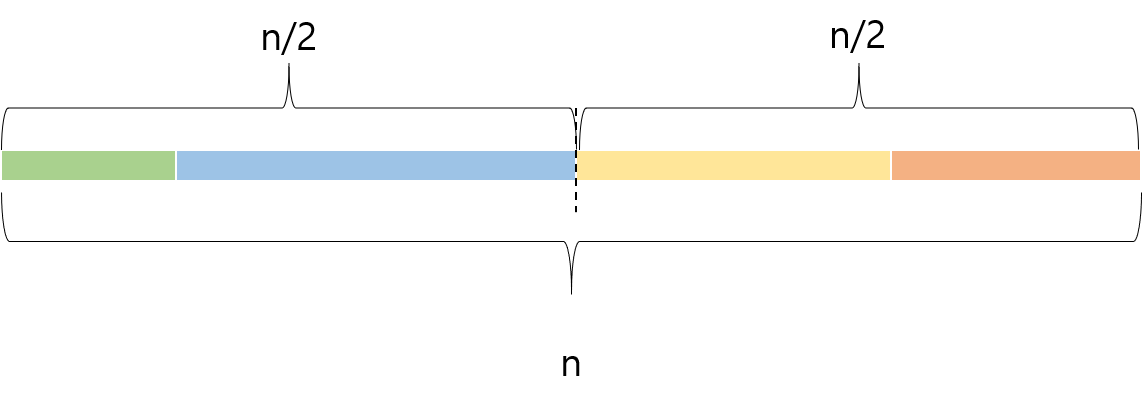
\includegraphics[scale=0.6]{figure1.png}
	\caption{Two charged magnets of each half}
\end{figure}

But my algorithm can not know which one is negative and which one is positive before the end. 
They just gathered the same charge magnets.
Test the any magnet from any group of each half.
Without loss of generallity, test green and yellow.
If green and yellow attract each other, then they have different charge. So union green with orange, and blue with yellow.
Then we have only two charge. Since we know that there are more positively charged magnet, whichever is bigger is the positive charged magnets.

{\bf Complexity}

Let's say time complexity of this algorithm is $T(n)$ where $n$ is the number of magnets.
Then because we do this in recursive method of each halves, following is the time complexity equation.
$T(n) = 2\cdot T(n/2) + O(1)$
Checking one element from one half with another element from another half takes $O(1)$, and unioning two union takes O(1).
Therfore, by the master theorem, $T(n)=n$.

{\bf Correctness}

My algorithm uses Union data structure. Make each magnet into nodes and store in the array list. I use array list to access to each element easily.
The algorithm is perfect if n is in the form $2^k$. 
When the list size is in the form $2k$, then split it by dividing into two, which is $k$, $k$ size respectively.
If the list size is in the form $2k+1$, then split it by dividing into two, which is $k$, $k+1$ size respectively.
When the list size is 1, there is nothing to do, so return the list itself.
Therefore, the algorithm is correct

\item 

{\bf Description}

My algorithm is to use the algorithm we used in class, but with a slight change.
\begin{figure}[hbt]
	\centering
	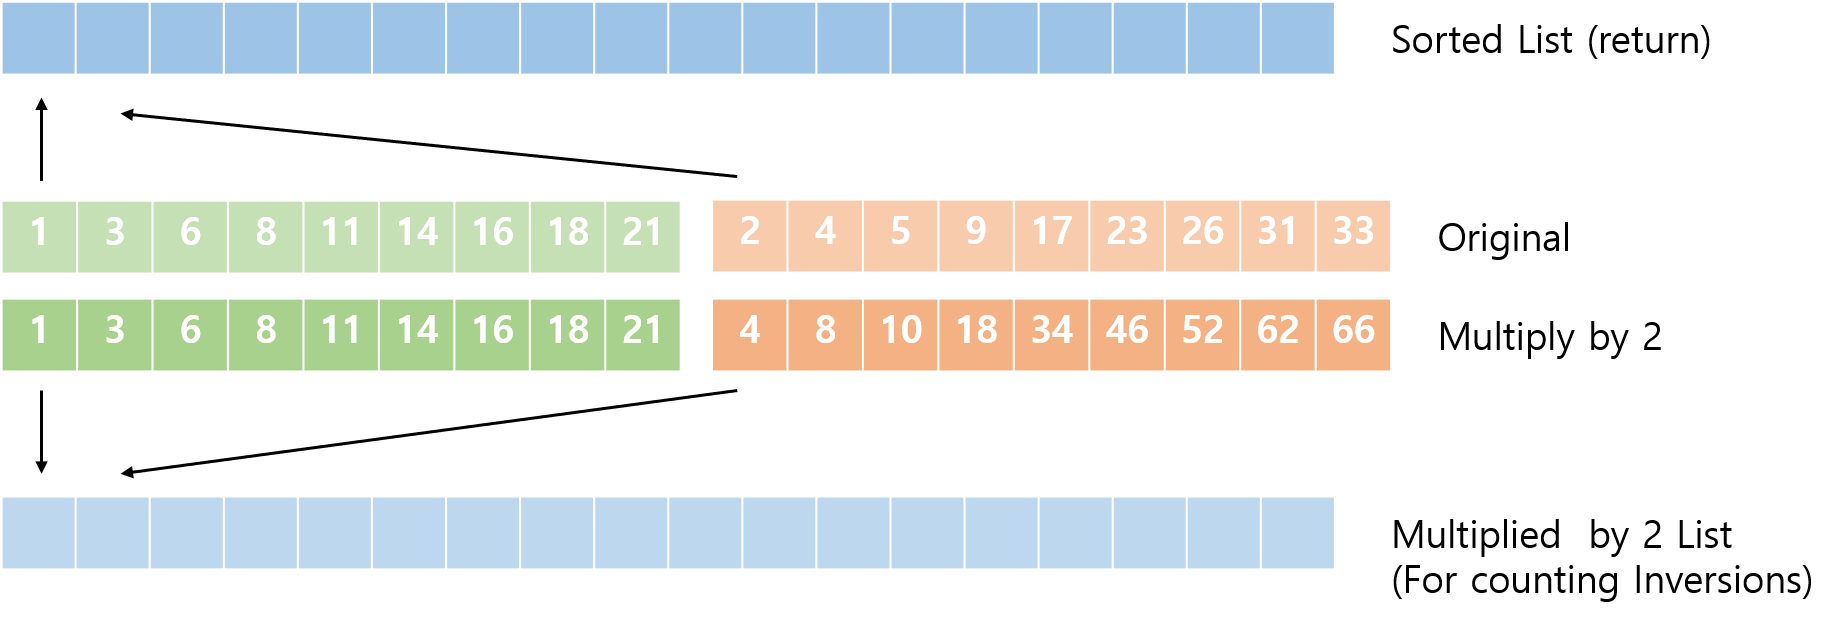
\includegraphics[scale=0.5]{figure2.png}
	\caption{asd}
\end{figure}

My algorithm will use recursive method, which returns sorted list and the number of inversions. 
We have sorted list of numbers.
We split this list into two halves.
Make a copy fo this list with 2 multiplied on the right half.(Figure 2)
Then for the original list, sort the list. 
We will return this sorted list for the recursion.
For the list that has right half multiplied by 2, sort the list and count the inversions.
The total inversion for this step is following.

For each element on the left list inserted to the blue list, the number of right elements that has been already inserted(this can be traced using integer variable).

Say this number of inversion is $k(List)$.
If we say $I(List)$ is the total inversions of the list, $I(List) = I(leftList) + I(rightList) + k(List)$.
We can get total number of inversion by recursively doing this.

{\bf Complexity}

If we say $T(n)$ is the time complexity of counting inversions of the n-size list, the time complexity equation follows.

$T(n) = 2 \cdot T(n/2) + O(n)$

We divide the list into two and count their inversion. This takes $2\cdot T(n/2)$.
We get sorted list after counting inversions of two halves.
Copying this list with multiplying 2 on the right half takes O(n) time.
Sorting the original list takes O(n) times.
Counting the inversion of multiplied list by sorting takes O(n) times.

Therefore by the master theorem, $T(n) = n \log n$.

{\bf Correctness}

The algorithm is correct when the size of the list is in form $2^k$.
In the recursive method, if the size of the list is form $2k$, then divide it into $k$,$k$ respectively, and continue the algorithm.
If the size of the list is in form $2k+1$, then divide it into $k$, $k+1$ respectively, and continue the algorithm.
If the size of the list is 1,  there is nothing to do so return that list.
Therefore, regardless of the size form of list, my algorithm is correct.


\end{enumerate}



\end{document}
